\documentclass{standalone}
\usepackage{tikz}
\usepackage{ctex,siunitx}
\setCJKmainfont{Noto Serif CJK SC}
\usepackage{tkz-euclide}
\usepackage{amsmath}
\usepackage{wasysym}
\usetikzlibrary{patterns, calc}
\usetikzlibrary {decorations.pathmorphing, decorations.pathreplacing, decorations.shapes,}
\begin{document}
\small
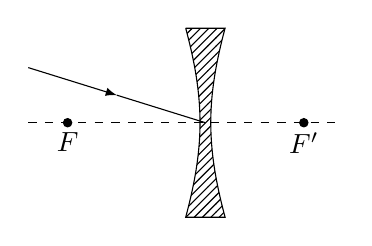
\begin{tikzpicture}[>=latex,scale=1]
  \draw [pattern=north east lines] (0,1.2) to [bend left=15] (0,-1.2)--(.5,-1.2) to [bend left=15](.5,1.2)--(0,1.2);
  \node at (-1.5,0)[below] {$F$};\node at (1.5,0)[below] {$F'$};
  \draw (-1.5,0) [fill=black]circle (1.5pt); \draw (1.5,0) [fill=black]circle(1.5pt);
  \draw [dashed] (-2,0)--(2,0);
  \draw [->](-2,.7)--(-1.75/2, .7/2);
  \draw (-1.75/2, .7/2)--(0.25, 0);
\end{tikzpicture}
\end{document}